


\subsection{Portfolio Construction}

\subsubsection{5 inputs to the portfolio construction process}
\begin{itemize}
\item Current portfolio: near certainty
\item Alphas: are often unreasonable and subject to hidden biases
\item Covariances
\item Active risk aversion: target level of active risk consistent with an active risk aversion
\item Transactions costs
\end{itemize}




\subsubsection{Refining alphas}
\begin{itemize}
\item Motivation: Most active managers construct portfolios subject to certain constraints, agreed upon with the client. These limits can make the portfolio less efficient, but they are hard to avoid.
    \begin{itemize}
    \item Not take short positions.
    \item Limit the amount of cash in the portfolio.
    \item Liquidity.
    \end{itemize}
\item Alphas can be adjusted so that they are in line with investor or manager's desires for risk control and various constraints.
\item Scale the alphas
\begin{align}
    \alpha &= \text{volatility} \cdot IC \cdot \text{Score} \notag \\
    &\quad \underset{\text{Residual risk}}{\uparrow}
    \end{align}
\[
\alpha \in [0 - z \times IC \times \text{Volatility}, 0 + z \times IC \times \text{Volatility}]
\]
    \begin{itemize}
    \item Score has a mean of zero and standard deviation of one.
    \item Information coefficient: Correlation between actual and forecasted outcomes.
    \item Example: An analyst regresses the returns of 200 stocks against the returns of a major market index. The resulting pool of 200 alphas has a residual risk of 25\% and an information coefficient of 8\%. If the alphas are normally distributed with a mean of 0\%, roughly how many stocks have an alpha greater than 4\% or less than -4\%?
    \item Answer:
    The interval of $\alpha$ is $[0 - 25\% \cdot 8\% \cdot z, 0 + 25\% \cdot 8\% \cdot z]$
\[
\rightarrow z = 2
\]
The total number of stocks is 200, so there are 10 alphas that are out of the range.
    \end{itemize}
\item Trim alpha outliers: very large positive or negative alphas can have undue influence.
    \begin{itemize}
    \item Closely examine all stocks with alphas greater in magnitude than three times the scale of the alphas.
    \end{itemize}
\item Neutralization: If our initial alphas imply an alpha for the benchmark, the neutralization process recenters the alphas to remove the benchmark alpha.
    \begin{itemize}
    \item Benchmark-and cash-neutral alphas: Adjusting the benchmark alpha to zero. The optimal position that uses benchmark will have a beta of one.
    \item Risk-Factor-neutral alphas: will include only information on the factors the manager can forecast.
   
    \end{itemize}
\item Neutralization:
    \begin{itemize}
        \item Benchmark-neutral alphas:
        \item Example 1: shift the alpha of the benchmark Major Market Index from 1.6 basis points to 0.
        
        \begin{table}[htbp]
            \centering
            \begin{tabular}{lccc}
                \toprule
                Stock & Beta & Alpha & Modified Alpha \\
                \midrule
                American Express & 1.21 & -1.14\% & -1.16\% \\
                AT\&T & 0.96 & 0.30\% & 0.29\% \\
                Chevron & 0.46 & 0.11\% & 0.10\% \\
                Coca Cola & 0.96 & -0.78\% & -0.79\% \\
                Disney & 1.23 & 0.60\% & 0.58\% \\
                Dow Chemical & 1.13 & 0.22\% & 0.20\% \\
                DuPont & 1.13 & -0.65\% & -0.67\% \\
                \bottomrule
            \end{tabular}
            \caption{American Express Modified Alpha = -1.14\% - 1.21 $\cdot$ 0.00016}
        \end{table}



        \item Example 2: You want to construct a portfolio so that all of the alphas are benchmark-neutral. Stock XYZ has a volatility of 30\%, an information coefficient of 0.2, and alpha of 90 basis points, and a beta of 1.94. The benchmark has an alpha of 3.7 basis points. What is the appropriate benchmark-neutral alpha for stock XYZ?
        \item Answer: modified benchmark-neutral alpha = 0.009-0.00037·1.94 = 0.0083
    \end{itemize}
\end{itemize}





\subsubsection{Active risk aversion}
\begin{itemize}
\item Determination of risk aversion:
    \begin{itemize}
    \item \(\text{Risk aversion}(\lambda_A) = \frac{IR}{2 \times \sigma_{\alpha}}\)
        \begin{itemize}
        \item \(\text{Utility (Value added)} = \alpha_p - \lambda_A \cdot \sigma_{\alpha}^2\)
        \end{itemize}
    \end{itemize}
    
\item Specific factor risk
    \begin{itemize}
    \item Decomposition of risk allows differing aversions to these different sources of risks.
        \begin{itemize}
        \item Utility = $\alpha_p - (\lambda_{A,CF} \cdot \sigma_{A,CF}^2 + \lambda_{A,SP} \cdot \sigma_{A,SP}^2)$
        \item Since specific risk arises from bets on specific assets, a high aversion to specific risk \textbf{reduces bets} on any one stock.
        \item For managers of multiple portfolios, aversion to specific risk can help \textbf{reduce dispersion}.
        \end{itemize}
    \end{itemize}
    
\end{itemize}



\subsubsection{Transaction costs}
\begin{itemize}
\item Transactions costs: are the costs of moving from one portfolio allocation to another.
    \begin{itemize}
    \item Rebalancing incurs transactions costs at that point in time. Transaction costs must be amortized over the investment horizon in order to determine the optimal portfolio adjustments.
    \end{itemize}
    
\item Revisions and rebalancing: fund manager should make the correct trade-off between expected active return, active risk, and transactions costs.
    \begin{itemize}
    \item If the manager is not sure of his or her ability to correctly specify the alphas, the active risk, and the transactions costs, less frequent revision may be a safeguard.
    \item The shorter time horizon for forecasting alphas, the larger amounts of noise. Rebalancing for very short horizons would involve frequent reactions to noise, not signal.
    \end{itemize}
\item Revisions and rebalancing:
\[
MCVA_n = \alpha_n - 2 \times \lambda_A \times \sigma_{\alpha} \times MCAR_n
\]
    \begin{itemize}
    \item MCVA (Marginal contribution to value added): shows how value added, as measured by risk-adjusted alpha, changes as the holding of the stock is increases.
    \item MCAR (Marginal contribution to active risk): measures the rate at which active risk changes as we add more of stock n. The change in value added also depends upon the impact (at the margin) on active risk of adding more of stock n.
    \end{itemize}
\item Revisions and rebalancing: In order to make rebalancing decision, we can compare the $MCVA_n$ for stock n to the transactions costs.

\[
MCVA_n = \alpha_n - 2 \times \lambda_A \times \sigma_{\alpha} \times MCAR_n
\]
\item No trade region:
\[
 - SC_n \leq MCVA_n \leq PC_n
\]
\[
2 \times \lambda_A \times \sigma_{\alpha} \times MCAR_n - SC_n \leq \alpha_n \leq PC_n + 2 \times \lambda_A \times \sigma_{\alpha} \times MCAR_n
\]
    \begin{itemize}
    \item Determination of the no-trade region: transactions costs, risk aversion, alpha and the riskiness of the assets.
    \end{itemize}
\end{itemize}






























\subsubsection{Portfolio construction techniques}
\begin{itemize}
\item Objective: maximizing active returns minus an active risk penalty.
\[
\text{Value added} = \alpha_p - \lambda_A \cdot \sigma_{\alpha}^2 - \text{transaction cost}
\]
    \begin{itemize}
    \item Screen(筛选)
    \item Stratification(分层)
    \item Linear programming(线性规划)
    \item Quadratic programming(二次规划)
    
    What procedures can we use to make the portfolio construction process robust in the presence of unreasonable and noisy inputs？

    \end{itemize}

\item Screen:

    \begin{center}
    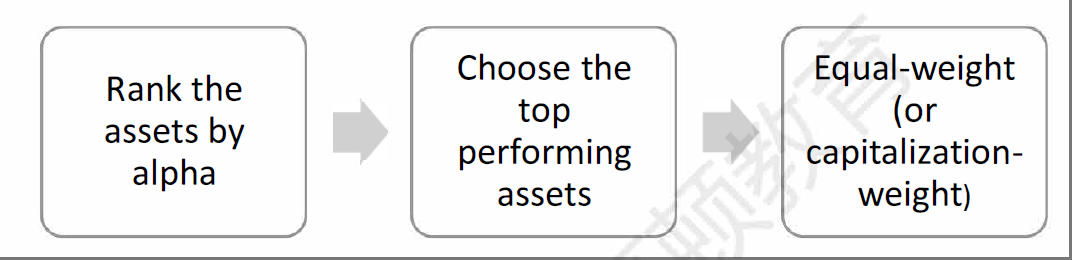
\includegraphics[width=0.9\textwidth]{images/scr.jpg}
    \end{center}       


    \begin{itemize}
    \item Divide the universe of assets into buy, hold, and sell decisions based on the rankings.
    \item Purchase any assets on the buy list not currently in the portfolio, and sell any assets in the portfolio that are on the sell list.
    \item Advantages:
        \begin{itemize}
        \item Simple; easy to understand and computerize
        \item Clear link between cause (buy, sell or hold) and effect (portfolio performance).
        \item The screen is robust. It depends solely on ranking so wild estimates of alphas will not alter the result.
        \item Enhances alphas by concentrating the portfolio in the high-alpha stocks
        \end{itemize}
    \item Risk control:
        \begin{itemize}
        \item Include a sufficient number of stocks and by weighting them to avoid concentration in any single stock.
        \item Transactions costs are limited by controlling turnover.
        \end{itemize}
    \item Disadvantages:
        \begin{itemize}
        \item Ignore all information in the alphas apart from the rankings.
        \item Excluded assets with lower alphas.
        \end{itemize}
    \end{itemize}
\item Stratification:
    \begin{itemize}
    \item Split the list of assets into mutually exclusive categories.
    \item Risk control: make sure that the portfolio has a representative holding in each category. Chosen well, the categories can lead to reasonable risk control while some important risk dimensions are excluded, risk control will fail.
    

    \begin{center}
        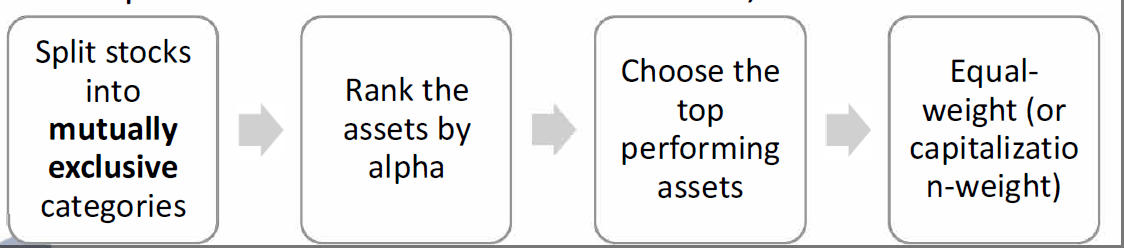
\includegraphics[width=0.9\textwidth]{images/wechat_2025-05-19_111641_221.jpg}
        \end{center}       

    \end{itemize}
\item Linear programming: characterizes assets along dimensions of risk, e.g. industry, size, volatility, and beta (without making the dimensions mutually exclusive).
    \begin{itemize}
    \item Advantages: takes all the information about alpha into account and controls risk by keeping the characteristics of the portfolio close to the characteristics of the benchmark.
    \item Disadvantages:
        \begin{itemize}
        \item Hard to produce portfolios with a prespecified number of stocks.
        \item The risk-control characteristics should not work at cross purposes with the alphas.
        \end{itemize}
    \end{itemize}
\item It also includes explicit transactions costs, a limit on turnover, and upper and lower position limits on each asset.

\item Objective of linear programming: maximize the portfolio's alpha less transactions costs while remaining close to the benchmark portfolio in the risk control dimensions.

\item Quadratic programming: explicitly considers alpha, risk, and transactions costs.
    \begin{itemize}
    \item Advantage: Including all the constraints and limitations one finds in a linear program.
    \item Disadvantage: A great many more inputs than the other portfolio construction techniques. More inputs mean more noise.
    \end{itemize}
\end{itemize}




























\subsubsection{Causes and Methods for Dispersion}
\begin{itemize}
\item Dispersion: fund managers run separate accounts for multiple clients but the portfolio returns are not identical.
    \begin{itemize}
    \item Dispersion is the difference between the maximum return and minimum return for separate account portfolios.
    \end{itemize}
    
\item Dispersion:
    \begin{itemize}
    \item Client-driven: constrains from clients
    \item Manager-driven: a lack of attention (separate accounts exhibit different betas and different factor exposures through lack of attention).
    \item If transactions costs were zero, dispersion would disappear, at no cost to investors.
    \end{itemize}
    
\end{itemize}



\subsection{Portfolio Risk: Analytical Methods}

\subsubsection{Portfolio VaR measures}
\begin{itemize}
\item Delta-normal model: all individual security returns are assumed normally distributed.
\item Traditional portfolio analysis: based on variances and covariances, which is why it is sometimes called the covariance matrix approach.
\item Individual VaR: The VaR of one component taken in isolation.

\begin{itemize}
    \item Transactions costs: are the costs of moving from one portfolio allocation to another.
        \begin{itemize}
        \item Rebalancing incurs transactions costs at that point in time. Transaction costs must be amortized over the investment horizon in order to determine the optimal portfolio adjustments.
        \end{itemize}
        
    \item Revisions and rebalancing: fund manager should make the correct trade - off between expected active return, active risk, and transactions costs.
        \begin{itemize}
        \item If the manager is not sure of his or her ability to correctly specify the alphas, the active risk, and the transactions costs, less frequent revision may be a safeguard.
        \item The shorter time horizon for forecasting alphas, the larger amounts of noise. Rebalancing for very short horizons would involve frequent reactions to noise, not signal.
        \end{itemize}
    \item Revisions and rebalancing:
    \begin{align*}
    MCVA_n &= \alpha_n - 2 \times \lambda_A \times \sigma_{\alpha} \times MCAR_n
    \end{align*}
        \begin{itemize}
        \item MCVA (Marginal contribution to value added): shows how value added, as measured by risk - adjusted alpha, changes as the holding of the stock is increases.
        \item MCAR (Marginal contribution to active risk): measures the rate at which active risk changes as we add more of stock n. The change in value added also depends upon the impact (at the margin) on active risk of adding more of stock n.
        \end{itemize}
    \item Revisions and rebalancing: In order to make rebalancing decision, we can compare the $MCVA_n$ for stock n to the transactions costs.
    \begin{align*}
    MCVA_n &= \alpha_n - 2 \times \lambda_A \times \sigma_{\alpha} \times MCAR_n
    \end{align*}
    \item No trade region:
    \begin{align*}
     - SC_n &\leq MCVA_n \leq PC_n \\
    2 \times \lambda_A \times \sigma_{\alpha} \times MCAR_n - SC_n &\leq \alpha_n \leq PC_n + 2 \times \lambda_A \times \sigma_{\alpha} \times MCAR_n
    \end{align*}
        \begin{itemize}
        \item Determination of the no - trade region: transactions costs, risk aversion, alpha and the riskiness of the assets.
        \end{itemize}
    \end{itemize}   

\item Diversified VaR: takes into account diversification benefits between components.
\item VaR for portfolio of two assets:
\item Undiversified VaR: is the sum of individual VaRs
\item Diversification benefit: the difference between the diversified VaR and the undiversified VaR which typically is shown in VaR reporting systems.
\item Example: A risk manager is evaluating a pairs trading strategy recently initiated by one of the firm's traders . The strategy involves establishing a long position in Stock A and a short position in Stock B. The following information is also provided:

1- day 99\% VaR of Stock A is USD 100 million

1-day 99\% VaR of Stock Bis USD 125 million

The estimated correlation between long positions in Stock A and Stock B is 0.8. Assuming that the returns of Stock A and Stock Bare jointly distributed, the 1-day 99\% VaR of the combined positions is closest to?

\item Answer:
\begin{align*}
    VaR_p &= z \cdot V \cdot \sqrt{w_1^2 \sigma_1^2 + w_2^2 \sigma_2^2 + 2 w_1 w_2 \sigma_1 \sigma_2 \rho_{12}} \\
    &= \sqrt{VaR_1^2 + VaR_2^2 + 2 VaR_1 VaR_2 \rho_{12}} \\
    &= \sqrt{100^2 + 125^2 + 2 \cdot (-0.8) \cdot 100 \cdot 125} = 75
    \end{align*}
    Since this is a pairs trading strategy with a long and a short position, the proper correlation to use is -0.8
    

\item Role of correlation on portfolio risk:
\[
\sigma_p = \sigma \sqrt{\frac{1}{N} + \left(1 - \frac{1}{N}\right)\rho}
\]
    \begin{itemize}
    \item All assets have the same risk.
    \item All correlations are the same.
    \item Equal weight is put on each asset.
    \end{itemize}
\end{itemize}


\subsubsection{VaR tools}
\begin{itemize}
\item Marginal VaR (MVaR): the change in portfolio VaR resulting from taking an additional dollar of exposure to a given component.
    \begin{align*}
    MVaR_i &= \frac{\partial VaR}{\partial (\text{investment})} = z \frac{\partial \sigma_p}{\partial w_i} \\
    &= z \frac{\text{cov}(R_i, R_p)}{\sigma_p} = z \cdot \sigma_i \cdot \rho_{ip} = z \cdot \beta_i \cdot \sigma_p = \frac{VaR_p \cdot \beta_i}{V_p}
    \end{align*}
    \begin{itemize}
    \item Example:There is a portfolio which is made up of two assets, stock ABC and stock XYZ. Assume the portfolio is valued at \$3 million and the 95\% VaR of the portfolio is \$257,738. Stock ABC has a beta of 0.6146. Please calculate the Marginal VaR of stock ABC.
    \item Answer:
    \[
MVaR_{ABC} = \frac{VaR_p \cdot \beta}{V_p} = \dfrac{0.6146 \cdot 257,738}{3,000,000} = 0.0528
\]
    \end{itemize}
    

\item Incremental VaR: is the change in VaR owing to a new position.
\[
\text{Full Incremental VaR} = VaR_{p + a} - VaR_p
\]
    \begin{itemize}
        \item The main \textbf{drawback} of this approach is that it requires a \textbf{full revaluation} of the portfolio VaR with the new trade (quite time - consuming for large portfolios).
        \item \textbf{Incremental VaR}: $\approx MVaR_i \cdot V_i$
    \end{itemize}
\item Component VaR: A partition of the portfolio VaR that indicates how much the portfolio VaR would change approximately if the given component was deleted.
\begin{align*}
    CVaR_i &= MVaR_i \times V_i \\
    &= MVaR_i \times w_i \times V_p = VaR_p \times \beta_i \times w_i \\
    \end{align*}
    Percentage contribution (\%) to VaR of component:
    \begin{align*}
    i &= \frac{CVaR_i}{VaR_p} = w_i \beta_i \\
    CVaR_1 + CVaR_2 + \cdots + CVaRn &= VaR_p \left( \sum_{i = 1}^{n} w_i \beta_i \right) = VaR_p
    \end{align*}
    \begin{itemize}
    \item Example 1:
    
    There is a portfolio which is made up of two assets, stock ABC and stock XYZ. Assume the portfolio is valued at \$3 million (Stock ABC \$2million, stock XYZ \$1milion) and the 95\% VaR of the portfolio is \$257,738. Marginal VaR of stock ABC is 0.0528. Please calculate the Component VaR of stock XYZ.
    \item Answer:
    \begin{align*}
         CVaR_{ABC} &= MVaR_i \times V_i \\
        &= 0.0528 \cdot 2,000,000 = 105,600 \\
        CVaR_{XYZ} &= 257,738 - 105,600 = 152,138
        \end{align*}
    \item Example 2:
    
    Please calculate the percent of contribution to VaR of each component.

    \begin{align*}
        i_{ABC} &= \dfrac{CVaR_{ABC}}{VaR} = \dfrac{105,600}{257,738} = 40.97\% \\
        i_{XYZ} &= \dfrac{CVaR_{XYZ}}{VaR} = \dfrac{152,138}{257,738} = 59.03\%
        \end{align*}
    \end{itemize}
\end{itemize}



\subsubsection{Risk management}
\begin{itemize}
\item Only taking risk into consideration $\rightarrow$ global minimum 

A manager can lower a portfolio VaR by:
    \begin{itemize}
    \item Lowering position with the highest marginal VaR.
    \item Adding position with the lowest marginal VaR.
    \end{itemize}
\item When the portfolio risk has reached a global minimum:
    \begin{itemize}
    \item All $MVaR_i$ must be equal.
    \item All betas must be equal.
    \end{itemize}
    
\item Taking return and risk into consideration $\to$ optimal portfolio

    \begin{itemize}
    \item Maximize the Sharpe ratio with VaR of the portfolio:
    \[
\dfrac{\overline{R}_p - \overline{R}_f}{VaR_p}
\]

    \item Lowering allocation to the position with the lowest excess expected return to marginal VaR.
    \item Adding allocation to the position with the highest excess expected return to marginal VaR.
    \[
\dfrac{R_i - R_f}{MVaR_i}
\]
    \end{itemize}
    
\item When the portfolio risk has reached a optimal portfolio:
\begin{itemize}
    \item All the ratios of $\dfrac{R_i - R_f}{MVaR_i}$ must be equal.
    \item All the ratios of $\dfrac{R_i - R_f}{\beta_i}$ must be equal.
\end{itemize}


\begin{center}
    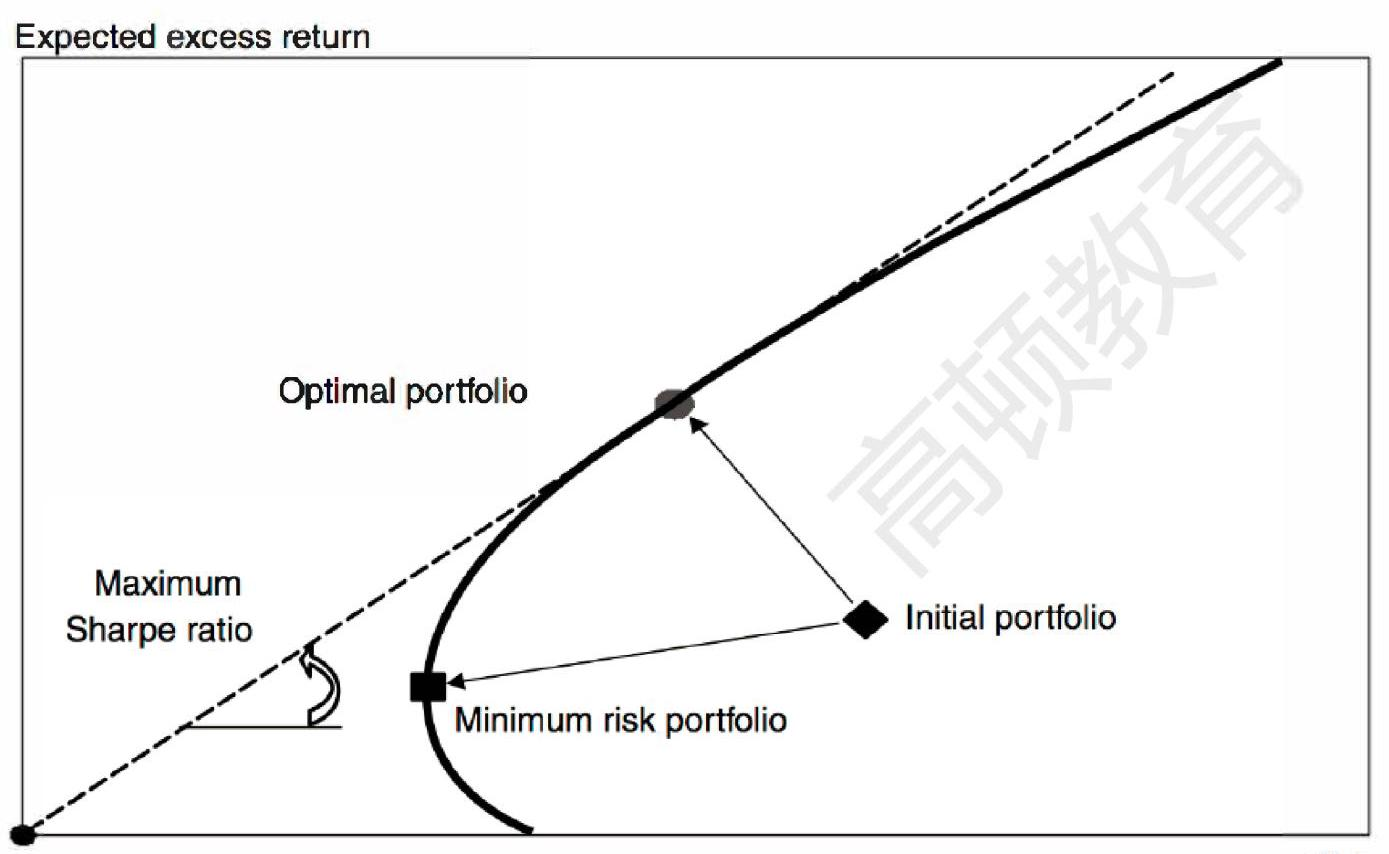
\includegraphics[width=0.9\textwidth]{images/Expected excess return.jpg}
    \end{center}     

\end{itemize}






\subsection{VaR and Risk Budgeting in Investment Management}


\subsubsection{Types of risks}
\begin{itemize}
\item Absolute risk vs. Relative risk
\item Policy-mix vs. Active-management
\item Funding risk
\end{itemize}



\subsubsection{Absolute vs. relative risk}
\begin{itemize}
\item Investment asset managers can have different perceptions of risk.
\item Absolute risk: is the risk of a dollar loss over the horizon.
\item Relative risk: is the risk of a dollar loss in a fund relative to its benchmark.
    \begin{itemize}
    \item If the excess return of the asset over the benchmark is normally distributed, VaR can be measured from the relative perspective:：$VaR_{\text{relative}} = z \cdot \sigma_{\alpha} \cdot V$
    \end{itemize}
    
\end{itemize}



\subsubsection{Policy-mix vs. active-management}
\[
R_{\text{asset}} = R_{\text{policy mix}} + R_{\text{active management}} = \sum_{i} w_i^b R_i^b + \sum_{i} (w_i R_i - w_i^b R_i^b)
\]
\begin{itemize}
\item Policy-mix risk: is the risk of a dollar loss owing to the policy mix selected by the fund. The risk from passive funds investment, this risk represents that of a passive strategy.
\item Active-management risk: is the risk of a dollar loss owing to the total deviations from the policy mix.
\item Most of the risk is due to the policy mix.
\item The active-management VaR is rather small.
\item The policy-mix VaR and active-management VaR do not add up to the total-asset VaR.
\end{itemize}



\subsubsection{Funding risk}
\begin{itemize}
\item Funding risk相关概念: surplus
\item $\Delta$ surplus
\item Surplus at risk
\item Confidence interval of surplus
\item A pension fund with defined benefits promises a stream of fixed payments to retires. If the assets are not sufficient to cover these liabilities, the shortfall will have to be made up by the fund's owner (provide additional contributions to the fund).
    \begin{itemize}
    \item Risk should be viewed in an asset liability management (ALM) framework.
    \item Funding risk: the value of assets will not be sufficient to cover the liabilities of the fund.
    \end{itemize}   
\end{itemize}



\subsubsection{Funding risk - surplus}
\begin{itemize}
\item Surplus: is the difference between the value of the assets and the liabilities.
    \begin{itemize}
    \item If liabilities consist mainly of nominal payments, their value will behave like a short position in a long-term bond.
    \begin{align*}
        \text{Surplus} &= \text{Assets} - \text{Liabilities} \\
        \Delta \text{Surplus} &= \Delta \text{Assets} - \Delta \text{Liabilities} = A \cdot R_A - L \cdot R_L \\
        R_{\text{surplus}} &= \frac{\Delta \text{Surplus}}{\text{Asset}} = \frac{\Delta \text{Asset}}{\text{Asset}} - \frac{\Delta \text{Liabilities}}{\text{Liabilities}} \times \frac{\text{Liabilities}}{\text{Asset}} \\
        &= R_{\text{asset}} - R_{\text{liability}} \frac{L}{A}
        \end{align*}
    \end{itemize}
\item Example ($\Delta$surplus):
    \begin{itemize}
    \item Neptune employee retirement fund had \$900 million in assets and \$800 million in liabilities. At the end of 2007, due to the huge crash, the investment in asset lost 50\% of their market value. The liabilities of the fund can be thought as a long-term debt with modified duration of 18. The interest rate declined 1.5\%. What was the surplus before the huge crisis and what was the change in the pension fund's surplus?
    \end{itemize}
    
\item Answer:
\begin{align*}
    \text{Surplus} &= \text{Assets} - \text{Liabilities} = 900 - 800 = 100 \\
    \Delta \text{Surplus} &= \Delta \text{Assets} - \Delta \text{Liabilities} \\
    &= 900 \times (-50\%) - (-\text{ModDur} \times \Delta y \times P) \\
    &= 900 \times (-50\%) - [-18 \times (-1.5\%) \times 800] = -666
    \end{align*}
\end{itemize}








\subsubsection{Funding risk - SaR}
\begin{itemize}
\item Surplus at risk (SaR):
    
\[\sigma_{\text{surplus}} = \sqrt{A^2 \cdot \sigma_A^2 + L^2 \cdot \sigma_L^2 - 2 \cdot A L \sigma_A \sigma_L \rho} \quad \text{(dollar term)} 
SaR = \left| E(\Delta \text{Surplus}) - Zc \cdot \sigma_{\text{surplus}} \right|\]


\item Example (SaR): Neptune employee retirement fund had \$900 million in assets and \$800 million in liabilities:

    \begin{tabular}{lcc}
    & Asset & Liabilities \\
    Return & 9\% & 6\% \\
    Volatility & 15\% & 20\% \\
    \end{tabular}

Assume that the correlation between asset return and liability growth is 0.5. Please compute 95\% surplus at risk.
\item Answer:
    \begin{align*}
    \text{Expected surplus growth} &= A \cdot R_A - L \cdot R_L \\
    &= 900 \cdot 9\% - 800 \cdot 6\% = 33 \text{ million} \\
    \sigma_{\text{surplus}} &= \sqrt{A^2 \cdot \sigma_A^2 + L^2 \cdot \sigma_L^2 - 2 \cdot A L \sigma_A \sigma_L \rho} \\
    &= \sqrt{900^2 \cdot 0.15^2 + 800^2 \cdot 0.20^2 - 2 \cdot 900 \cdot 800 \cdot 0.15 \cdot 0.2 \cdot 0.5} \\
    &= 149 \\
    95\% SaR &= \left| 33 - 1.645 \cdot 149 \right| = 212.11 \text{ million}
    \end{align*}
\end{itemize}












\subsubsection{Funding risk - Confidence interval}
\begin{itemize}
\item The confidence interval for expected end-of-year surplus
\begin{align*}
&[E(\text{Surplus}_1) - z \times \sigma_s, \ E(\text{Surplus}_1) + z \times \sigma_s] \\
&E(\text{Surplus}_1) = \text{Surplus}_0 + E(\Delta \text{surplus})
\end{align*}

\item Example (Confidence interval): information to the advisor or a pension fund that currently invests in government and corporate bonds:

\begin{tabular}{lcc}
    \toprule
    Pension & Assets & Liabilities \\
    \midrule
    Amount (EUR million) & 200 & 180 \\
    Expected annual growth rate & 5\% & 7\% \\
    \bottomrule
\end{tabular}

Assuming that the volatility of surplus in dollars is EUR 36 million, what is the lower bound of the 95\% confidence interval for the expected end-of-year surplus?

\item Answer:

    \begin{itemize}
    \item $\text{Surplus}_0 = 200 - 180 = 20 \text{million}$
    \item $\Delta \text{surplus} = 200 \times 5\% - 180 \times 7\% = -2.6 \text{million}$
    \item $E(\text{Surplus}) = \text{Surplus}_1 = \text{Surplus}_0 + \Delta \text{surplus} = 20 - 2.6 = 17.4 \text{million}$
    \item Lower bound of confidence interval:
    $E(\text{Surplus}) - z \times \sigma_s = 17.4 - 1.96 \times 36 = -53.16 \text{million}$
    \end{itemize}

\end{itemize}







\subsubsection{Funding risk}
\begin{itemize}
\item Sponsor risk: surplus risk can be extended to the risk to the owner of the fund who ultimately bear responsibility for the pension fund.
    \begin{itemize}
    \item Economic risk: is the variation in the total economic earnings of the plan sponsor. (if the firm enjoys greater operating profits, the surplus risk may be less of a concern.)
    \item Cash-flow risk: is the risk of year-to-year fluctuations in contributions to the pension fund.
    \end{itemize}
\end{itemize}











\subsubsection{VaR applications to investment management}
\begin{itemize}
\item Sell side versus buy side:

\begin{tabular}{@{}l l l @{}}
    \toprule
    Characteristic & Sell Side (Banks) & Buy Side (Investment Management) \\
    \midrule
    Horizon & Short-term (1 day, intraday) & Long-term (month, quarter, years) \\
    Turnover & Rapid & Slow \\
    Leverage & High & Low \\
    Risk measures & VaR, Stress test & Asset allocation, Tracking error \\
    Risk controls & Position limits, VaR limits, Stop-loss rules & Diversification, Benchmarking, Investment guidelines \\
    \bottomrule
\end{tabular}

\item Investment process of large investors (e.g. pension funds)
    \begin{itemize}
    \item Step One: strategic, long-term asset-allocation study
        \begin{itemize}
        \item Based on mean-variance portfolio optimization
        \item Determines the amounts to be invested in various asset classes
        \end{itemize}
    \item Step Two: delegate fund managers
        \begin{itemize}
        \item Conduct performance evaluation periodically relative to their benchmark
        \item Investment guidelines and some additional restrictions: duration, maximum deviations from equity-sector weights, maximum amounts of foreign currency to hedge, etc.
        \end{itemize}
    \item Institutions exposed to a diversity of risk , to complex financial instruments, and to changing positions should benefit from VaR risk management systems.
        \begin{itemize}
        \item Take diversification into account.
        \item A need for stronger, centralized risk management systems (Financial instruments are becoming more complex).
        \item Most investment portfolios are dynamic.
        \end{itemize}
    \end{itemize}
\item Hedge fund: poses special risk measurement problems.
    \begin{itemize}
    \item High leverage
    \item Lack of transparency
    \item Heterogeneous
        \begin{itemize}
        \item Some groups have greater turnover than traditional investment managers $\to$risk management systems similar to the bank
        \end{itemize}
    \end{itemize}
\end{itemize}






\subsubsection{Using VaR to monitor and control risks}
\begin{itemize}
\item Check compliance
    \begin{itemize}
    \item Unauthorized investment: some securities may be prohibited because of their risks or for other reasons (e.g., political or religious). But some fund managers sometimes trade in and out of unauthorized investment before the client realized what happened.
    \end{itemize}
\item Monitor risk
    \begin{itemize}
    \item Fund managers and investors would notice a sudden jump in the reported VaR of the fund. The reason may be:
        \begin{itemize}
        \item A manager taking more risk.
        \item Different managers taking similar bets.
        \item More volatile markets.
        \end{itemize}
    \item VaR can be reverse engineered to understand where risk is coming from using VaR tools (e.g., component VaR, marginal VaR).
    \end{itemize}
    
\end{itemize}



\subsubsection{Risk budgeting}
\begin{itemize}
\item Risk budgeting: the process of decomposing the aggregate risk of a portfolio into its constituents, using these risk measures to allocate assets, setting limits in terms of these measures, and then using the limits to monitor the asset allocations and portfolio managers


\begin{center}
    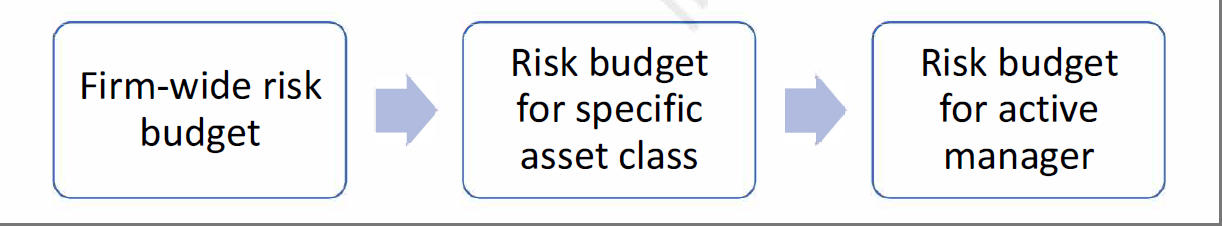
\includegraphics[width=0.9\textwidth]{images/riskbudgeting.jpg}
    \end{center}     

\end{itemize}



\subsubsection{Risk budgeting - across asset classes}
\begin{itemize}
\item Example 1: a firm's management might set a annual return volatility target equal to 10\%. If the firm has 1000 million in assets under management and assuming the returns are normally distributed, at a 99\% confidence level.

\begin{table}[h]
    \centering
    \caption{Risk budgeting across asset classes at 99\% (millions)}
    \begin{tabular}{lcccc}
        \toprule
        Asset & Weight & Volatility & Principal & Risk Budget \\
        \midrule
        U.S. stocks & 52.5\% & 15.1\% & \$525 & \$184 \\
        Non-U.S. stocks & 10.4\% & 16.7\% & \$104 & \$41 \\
        U.S. bonds & 12.25\% & 7.3\% & \$122 & \$21 \\
        Non-U.S. bonds & 24.9\% & 10.9\% & \$249 & \$63 \\
        Portfolio & 100\% & 10.0\% & \$1000 & \$233 \\
        \bottomrule
    \end{tabular}
\end{table}

\begin{align*}
VaR_{\text{US stocks}} &= 2.326 \cdot 0.151 \cdot 525 = 184 \\
\text{Undiversified } VaR &= \sum \text{Risk Budget} = \$309 > \$233
\end{align*}

\item Example 2: the current portfolio fund manager Henry holding is a €100 million investment with 10\% volatility. The risk budget he set is €40million at 99\% confidence level. Which investment should he add into current portfolio can keep his risk budget?

\begin{tabular}{@{}lccc@{}}
    \toprule
    & Return volatility & Correlation with current portfolio & Value \\
    \midrule
    Emerging market stocks & 15\% & -0.14 & 100million \\
    Investment grade bonds & 8.5\% & 0.8 & 100million \\
    \bottomrule
\end{tabular}

\begin{align*}
VaR_{\text{stock}} &= 15\% \cdot 100 \cdot 2.326 = 34.89 \text{million} \\
VaR_{\text{bond}} &= 8.5\% \cdot 100 \cdot 2.326 = 19.77 \text{million} \\
VaR_{\text{current}} &= 10\% \cdot 100 \cdot 2.326 = 23.26 \text{million}
\end{align*}

If adding emerging market stocks into portfolio:
\[
VaR_{\text{new}} = \sqrt{34.89^2 + 23.26^2 - 2 \cdot 34.89 \cdot 23.26 \cdot 0.14} = 39.13 \text{million}
\]
If adding investment grade bonds into portfolio:
\[
VaR_{\text{new}} = \sqrt{19.77^2 + 23.26^2 + 2 \cdot 19.77 \cdot 23.26 \cdot 0.8} = 40.84 \text{million}
\]

\end{itemize}



\subsubsection{Risk budgeting - across active managers}
\begin{itemize}
\item A greater risk budget should be allocated to managers with better performance, as measured by the IR criterion.
\item Weight of portfolio managed by manager i:
\[
w_i = \frac{\frac{IR_i}{TE_i}}{\frac{IR_p}{TE_p}} = \frac{\frac{\alpha_i}{TE_i^2}}{\frac{\alpha_p}{TE_p^2}}
\]

Assume that the deviations for each manager are independent of each other

TE: track error
\item Example: PERF wants to allocate \$525 million to a pool of active managers so as to maximize the information ratio of the fund subject to an overall tracking error (TE) of 4\%.
\item Please calculate the weight of portfolio and relative risk budget which is allocated to manager 1.

\begin{center}
\begin{tabular}{@{}lcc@{}}
    \toprule
    & $TE_i$ & $IR_i$ \\
    \midrule
    Manager 1 & 6\% & 0.6 \\
    Manager 2 & 6\% & 0.4 \\
    Portfolio & 4\% & 0.72 \\
    \bottomrule
\end{tabular}
\end{center}

\item Answer:

\begin{table}[h]
    \centering
    \caption{Risk Budgeting for Portfolio Managers}
    \begin{tabular}{@{}lccccc@{}}
        \toprule
        & $TE_i$ & $IR_i$ & Weight & Allocated Principal & \cellcolor{white}\makecell{Relative risk budget \\ (99\% confidence level)} \\
        \midrule
        Manager 1 & 6\% & 0.6 & 55.6\% & \$291 & \$40.6 \\
        Manager 2 & 6\% & 0.4 & 37.04\% & \$194 & \$27.1 \\
        Index & 0\% & 0 & 7.36\% & \$40 & \$0 \\
        Portfolio & 4\% & 0.72 & 100\% & \$525 & \$48.85 \\
        \bottomrule
    \end{tabular}
\end{table}


\begin{align}
Weight_{\text{manager 1}} &= \dfrac{\frac{IR_i}{TE_i}}{\dfrac{IR_p}{TE_p}} = \dfrac{\dfrac{0.6}{6\%}}{\dfrac{0.72}{4\%}} = 55.6\% \\
\text{Amount} &= 55.6\% \times 525 \text{million} = 291.9 \text{million}
\end{align}

\[
\text{Relative risk budget} = z \cdot \sigma_{\alpha} \cdot V = 2.326 \times 291 \times 6\% = 40.61 \text{million}
\]


\item The residual weight is allocated to the index.
\end{itemize}



\subsection{Risk Monitoring and Performance Measurement}



\subsubsection{VaR vs. Tracking error}
\begin{itemize}
\item VaR: the maximum dollar loss associated with a given level of statistical confidence over a given period of time.
    \begin{itemize}
    \item To achieve targeted levels of dollar VaR, owners of capital allocate capital among asset classes.
    \end{itemize}
\item Tracking error: gauges the risk profile relative to a benchmark (standard deviation of excess returns).
    \begin{itemize}
    \item Tracking error is used to describe the extent to which the investment manager is allowed latitude to differ from the index.
    \end{itemize}
\end{itemize}



\subsubsection{Three-legged risk management stool}
\begin{center}
    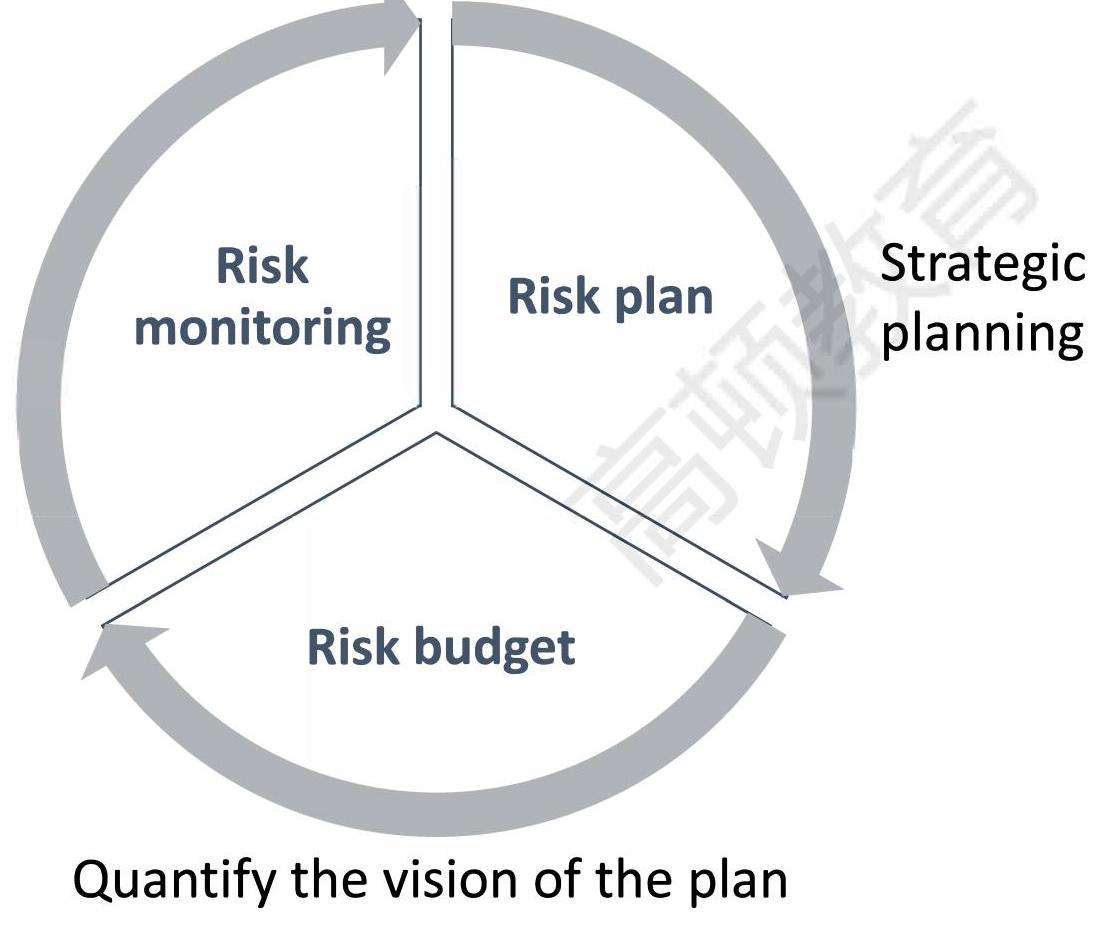
\includegraphics[width=0.9\textwidth]{images/Quantify the vision of the plan.jpg}
    \end{center}     

\begin{itemize}
\item Risk plan
    \begin{itemize}
    \item Set expected return and expected volatility (e.g., VaR and tracking error)
    \item Define the bright line between those events that are merely disappointing and those that inflict serious damage.
    \item Paint a vision of how risk capital will be deployed to meet the organization's objectives.
    \item The risk plan should identify critical dependencies that exist inside and outside the organization.
    \end{itemize}
\item Risk budget
    \begin{itemize}
    \item The risk budget should quantify the vision of the risk plan
        \begin{itemize}
        \item Using mean-variance optimization to determine appropriate weights for each class (expected returns, risks, and covariances, organization's strategic objectives and risk tolerances).
        \item Ensure ROE and RORC must exceed some minimum levels.
        \item Simulate the performance of a portfolio (e.g. downside scenarios)
        \end{itemize}
    \end{itemize}
\item Risk monitoring
    \begin{itemize}
    \item Risk capital is a scarce commodity, so monitoring controls should exist to ensure that risk capital is used in a manner consistent with the risk budget.
        \begin{itemize}
        \item Risk monitoring is required to ensure that material deviations from risk budget are detected and addressed in a timely fashion.
        \end{itemize}
    \end{itemize}
\end{itemize}



\subsubsection{Risk management units (RMUs)}
\begin{itemize}
\item RMUs:
    \begin{itemize}
    \item Role: oversee the risk exposures of portfolios and ensure that such exposures are authorized and in line with risk budgets.
    \item Must be established independently from the business areas and operate as a controlling or monitoring function.
        \begin{itemize}
        \item have an independent reporting line to senior management.
        \end{itemize}
    \item Gathers, monitors, analyzes, and distributes risk data to managers, clients, and senior management in order to better understand and control risk.
    \item Should not manage risk, but rather measure risk.
    \item Watches trends in risk as they occur and identifies unusual events to management in a timely fashion.
    \item Identifies and develops risk measurement and performance attribution analytical tools
    \item Provides tools for both senior management and individual portfolio management to better understand risk in individual portfolios and the source of performance.
    \item Helps ensure that transactions are authorized in accordance with management direction and client expectations.
    \end{itemize}
    
\end{itemize}



\subsubsection{Liquidity Considerations}
\begin{itemize}
\item Liquidity duration: the number of days required to liquidate any given security.
\[
LD_i = \frac{Q_i}{0.15 \cdot V_i}
\]
LD: liquidity duration statistic for security\\
15\%: we do not wish to exceed 15\% of the daily volume in that security to avoid a \textbf{material adverse earning impact}.\\
Q: number of shares held in security\\
V: daily volume of the security
\end{itemize}



\subsubsection{Performance measurement}
\begin{itemize}
\item Objectives of performance measurement tools:
    \begin{itemize}
    \item To determine whether a manager generates consistent excess risk-adjusted performance to a benchmark.
    \item To determine whether a manager generates superior riskadjusted performance to the peer group.
    \item To determine whether the returns achieved are sufficient to compensate for the risk assumed in cost/ benefit terms.
    \item To identifying those managers whose processes generate high-quality excess risk-adjusted returns.
    \end{itemize}
\item Tool 1: The green zone - For prior week, month, year: calculate normalized returns (excess returns) and tracking error. Then, Compare actual outcomes to target outcomes.
\item Policy decisions about deviations:
    \begin{itemize}
    \item Green zone: An acceptable amount of deviation.
    \item Yellow zone: Unusual events that are expected to occur with some regularity.
    \item Red zone: Truly unusual events and requiring immediate follow-up.
    \end{itemize}
\item Tool 2 - Attribution of returns
\item Tool 3 - T he Sharpe and information ratios
\item Tool 4 - Alpha versus the benchmark
\item Tool 5 - Alpha versus the peer group
\end{itemize}




\subsection{Portfolio Performance Evaluation}



\subsubsection{Return calculation}
\begin{itemize}
\item Time-weighted returns: The compound return that \$1 initially invested in the portfolio over a stated measurement period.
\begin{align*}
(1 + R_G)^n &= (1 + R_1)(1 + R_2)(1 + R_3)\cdots(1 + R_n) \\
1 + R_G &= [(1 + R_1)(1 + R_2)(1 + R_3)\cdots(1 + R_n)]^{1/n}
\end{align*}
\item Each return has an equal weight in the geometric average. The geometric average is referred to as a time-weighted average.
\item Dollar-weighted returns: accounts for the timing and amount of all cash flows into and out of the portfolio.
\item Calculation of DWR: similar to IRR.
\[
CF_0 + \frac{CF_1}{1 + DWR} + \cdots + \frac{CF_n}{(1 + DWR)^n} = 0
\]
\item Example:

\begin{table}[h]
    \centering
    \caption{Stock Investment Cash Flows}
    \begin{tabular}{@{}lc@{}}

        Time & Outlay / Proceeds \\
        \midrule
        0 & \$50 to purchase first share \\
        1 & \$53 to purchase second share a year later \\
        1 & \$2 dividend from initially purchased share \\
        2 & \$4 dividend from the 2 shares in the second year, plus \$108 received from selling both shares at \$54 each \\
        \bottomrule
    \end{tabular}
\end{table}


\text{TWR: }
\begin{align*}
R1 &= \frac{53 + 2 - 50}{50} = 10\% \\
R2 &= \frac{108 + 4 - 53 \cdot 2}{53 \cdot 2} = 5.66\% \\
TWR &= \sqrt{(1 + R1)(1 + R2)} - 1 = 7.8\%
\end{align*}

\text{DWR: }
\[
0 = -50 + \frac{-53 + 2}{1 + DWR} + \frac{108 + 4}{(1 + DWR)^2} \rightarrow DWR = 7.117\%
\]


\begin{table}[h]
    \centering
    \caption{Calculation Steps for IRR}
    \begin{tabular}{@{}lc@{}}
        \toprule
        Steps & Display \\
        \midrule
        {[}CF{]} & CF0=0.0000 \\
        {[}2nd{]}{[}CE/C{]} & CF0=0.0000 (Clear previous works) \\
        {[}50{]}{[}+|-{]}{[}ENTER{]} & CF0=-50.0000 \\
        {[}$\downarrow${]}{[}51{]}{[}+|-{]}{[}ENTER{]} & C01=-51.0000 \\
        {[}$\downarrow${]}{[}{[}$\downarrow${]}{[}112{]}{[}ENTER{]} & C02=112 \\
        {[}IRR{]}{[}CPT{]} & IRR=7.117\% \\
        \bottomrule
    \end{tabular}
\end{table}

计算器上的F表示frequency，即这笔现金流出现了几次由于题目中现金流都是只出现一次，默认为1往下翻即可。


\item DWR: If more funds to invest:
    \begin{itemize}
    \item Before favorable time: the dollar-weighted rate of return will tend to be elevated (higher/increased).
    \item Before unfavorable time: the dollar-weighted rate of return will tend to be depressed (lower/decreased).
    \end{itemize}
\item TWR: The use of the time-weighted return removes distortions of fund investing, providing a better measure of a manager's ability to select investments over the period.
\end{itemize}



\subsubsection{Risk-adjusted performance measures}
\begin{itemize}
\item Sharpe ratio: divides average portfolio excess return over the sample period by the standard deviation of returns (total risk) over that period.
\[
\text{Sharpe Ratio} = \frac{\overline{R_p} - \overline{R_f}}{\sigma_p}
\]
\item Treynor ratio: like the Sharpe ratio, Treynor's measure gives excess return per unit of risk, but it uses systematic risk instead of total risk.
\[
\text{Treynor Ratio} = \frac{\overline{R_p} - \overline{R_f}}{\beta_p}
\]
\item Sharpe ratio vs. Treynor ratio:
    \begin{itemize}
    \item Well-diversified portfolio: performance evaluation using 
    
    Sharpe ratio and Treynor ratio will give the same ranking result.
    \item Not well-diversified portfolio: it may be ranked relatively higher using Treynor ratio than using Sharpe ratio.
    \end{itemize}
\item Jensen's alpha: is the average return on the portfolio over and above that predicted by the CAPM, given the portfolio's beta and the average market return.
\[
\alpha_p = \overline{r_p} - \left[\overline{r_f} + \beta_p (\overline{r_m} - \overline{r_f})\right]
\]
\item Information ratio: measures excess return over benchmark per unit of risk.
\[
IR = \frac{\alpha_p}{\sigma(\alpha_p)}
\]
    \begin{itemize}
    \item A higher information ratio indicates better performance.
    \end{itemize}
    
\item Modigliani-squared measure ($m^2$):

    \begin{itemize}
    \item we adjust the return of portfolio to the same standard deviation as the index. Because the market index and portfolio have the same standard deviation, we can compare their performance simply by comparing returns.
    \end{itemize}
\[
M^2 = \frac{\sigma_m}{\sigma_p}(R_p - R_f) - (R_m - R_f)
\]

\begin{center}
    \includegraphics[width=0.4\textwidth]{images/modi.jpg}
    \end{center}     

\item Example: consider the following data for a particular sample period

\begin{table}[h]
    \centering
    \caption{Portfolio and Market Metrics}
    \begin{tabular}{@{}lcc@{}}
        \toprule
        & Portfolio P & Market M \\
        \midrule
        Average return & 35\% & 28\% \\
        Beta & 1.2 & 1 \\
        Standard deviation & 42\% & 30\% \\
        Tracking error & 18\% & 0 \\
        \bottomrule
    \end{tabular}
\end{table}
\item Please calculate Sharpe, Jensen (alpha), Treynor, information ratio and $m^2$. The T-bill rate during the period was 6\%. By which measures did portfolio outperform the market.
\item Answer:
\begin{table}[h]
    \centering
    \caption{Performance Metrics Comparison}
    \begin{tabular}{@{}lcc@{}}
        \toprule
        & Portfolio P & Market M \\
        \midrule
        Sharpe ratio & 0.6905 & 0.7333 \\
        Treynor ratio & 0.2417 & 0.22 \\
        Jensen’s alpha & 0.026 & 0 \\
        Information ratio & 0.3889 & 0 \\
        $M^2$ & -0.0129 & 0 \\
        \bottomrule
    \end{tabular}
\end{table}
\end{itemize}



\subsubsection{Market timing}
\begin{itemize}
\item Market timing involves shifting funds between a market-index portfolio and a safe asset depending on whether the market index is expected to outperform the safe asset.
\item Assume fund manager holds only the market-index portfolio and T-bills.
\item No market timing (the weight of the market are constant)
\[
R_p - R_f = a + b(R_m - R_f) + e_p
\]
\begin{center}
    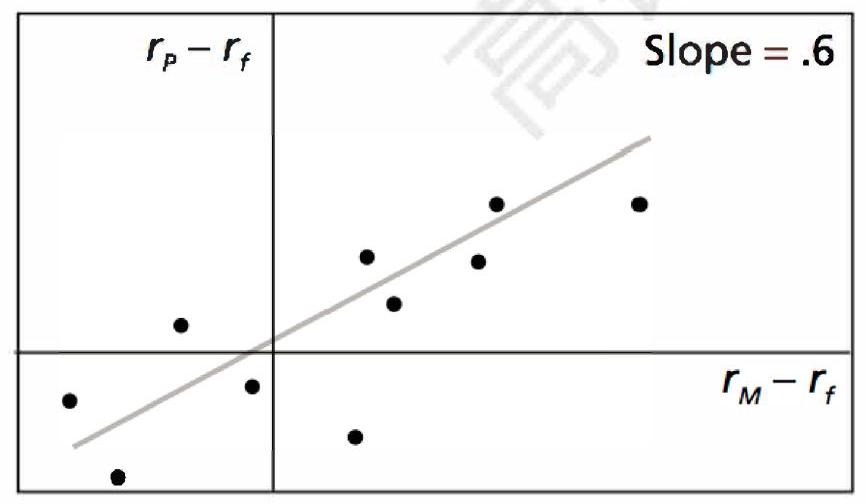
\includegraphics[width=0.4\textwidth]{images/No market timing.jpg}
    \end{center}     
\item With market timing (Treynor and Mazuy)
\[
R_p - R_f = a + b(R_m - R_f) + c(R_m - R_f)^2 + e_p
\]
\begin{center}
    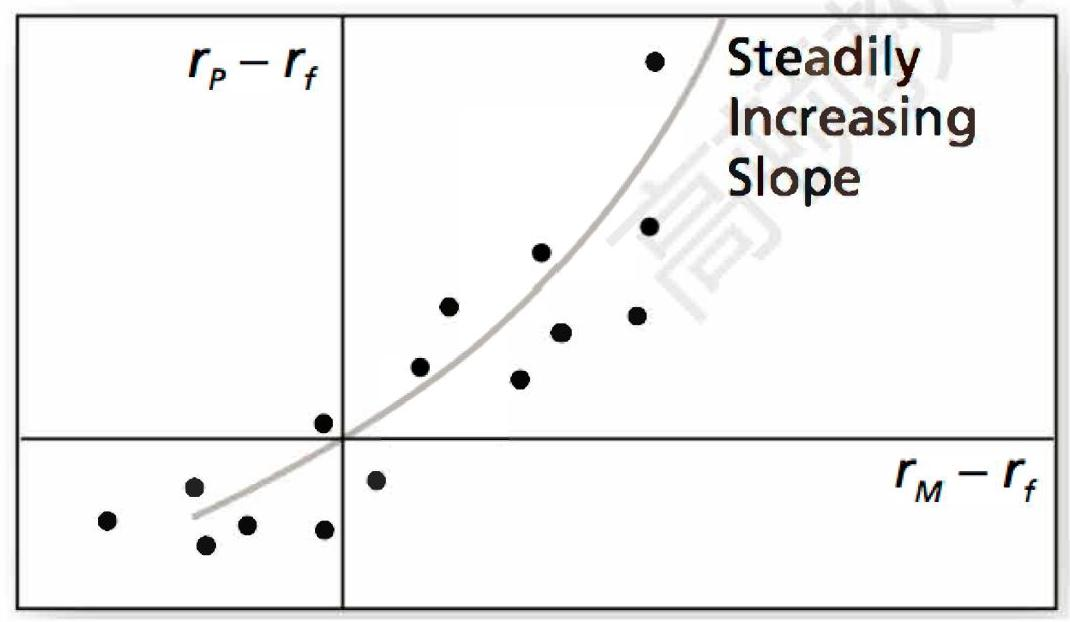
\includegraphics[width=0.4\textwidth]{images/With market timing.jpg}
    \end{center}    


\item With market timing (Henriksson and Merton): the beta of the portfolio takes a large value if the market is expected to do well and a small value otherwise.
\[
R_p - R_f = a + b(R_m - R_f) + c(R_m - R_f)D + e_p
\]
    \begin{itemize}
    \item D is a dummy variable with O for bear markets (RM < Rf) and 1 for bull markets (RM > Rf) .
    \end{itemize}
    \begin{center}
        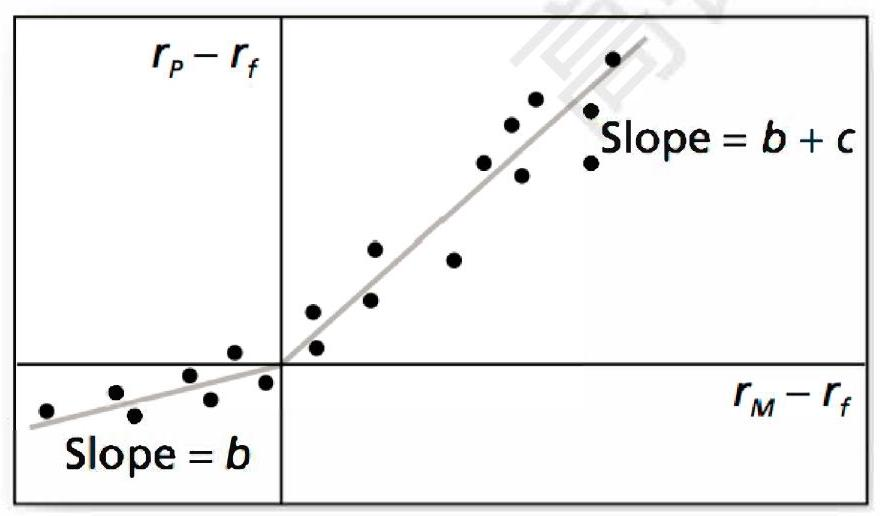
\includegraphics[width=0.4\textwidth]{images/Henriksson.jpg}
        \end{center}    
    
\item Call option model: The perfect foresight is equivalent to holding a call option on the equity portfolio. The rate of return is at least the risk-free rate.
\item Suppose that the market index currently is at $S_0$ and that a call option on the index has an exercise price of $X=S_0（1+R_f）$

\begin{table}[H]
    \centering
    \caption{Option Payoff Analysis}
    \begin{tabular}{@{}lcc@{}}
        \toprule
        & $S_T < X$ & $S_T \geq X$ \\
        \midrule
        Bills & $S_0(1 + R_f)$ & $S_0(1 + R_f)$ \\
        Call & 0 & $S_T - X$ \\
        Total & $S_0(1 + R_f)$ & $S_T$ \\
        \bottomrule
    \end{tabular}
\end{table}
\end{itemize}



\subsubsection{Performance attribution}
\begin{itemize}
\item The attribution method explains the difference in returns between a managed portfolio, P, and a selected benchmark portfolio, B, called the bogey.
\item Example: The portfolio return over the month is 5.34\%
\begin{table}[H]
    \centering
    \caption{Bogey Performance}
    \begin{tabular}{@{}lcc@{}}
        \toprule
        & Benchmark weight & Return of index during month(\%) \\
        \midrule
        Equity (S\&P500) & 60\% & 5.81 \\
        Bonds (Barclays aggregate index) & 30\% & 1.45 \\
        Cash (money market) & 10\% & 0.48 \\
        \bottomrule
    \end{tabular}
\end{table}

Alpha= 5.34\% - (60\%·5.81\%+30\%·1.45\%+10\%·0.48\%) = 1.37\%

\item Three components in attribution system:
    \begin{itemize}
    \item Asset allocation: Broad asset market allocation choices across equity, fixed-income, and money markets.
    \item Selection:
        \begin{itemize}
        \item Industry (sector) choice within each market.
        \item Security choice within each sector.
        \end{itemize}  
    \end{itemize}

\item Example (cont.):
\begin{table}[h]
    \centering
    \caption{Portfolio and Benchmark Performance}
    \begin{tabular}{@{}lccc@{}}
        & Equity & Bonds & Cash \\
        \midrule
        Return of index during month(\%) & 5.81 & 1.45 & 0.48 \\
        Benchmark weight & 60\% & 30\% & 10\% \\
        Portfolio performance (\%) & 7.28 & 1.89 & 0.48 \\
        Actual weight & 70\% & 7\% & 23\% \\
        \bottomrule
    \end{tabular}
\end{table}

\[
\begin{array}{lc}
\text{Contribution from asset allocation} & (W_{Pi} - W_{Bi}) \times R_{Bi} \\
\text{+ Contribution from security selection (selection)} & (R_{Pi} - R_{Bi}) \times W_{Pi} \\
\text{= Total contribution from asset class i} & W_{Pi}R_{Pi} - W_{Bi}R_{Bi}
\end{array}
\]

    \begin{center}
    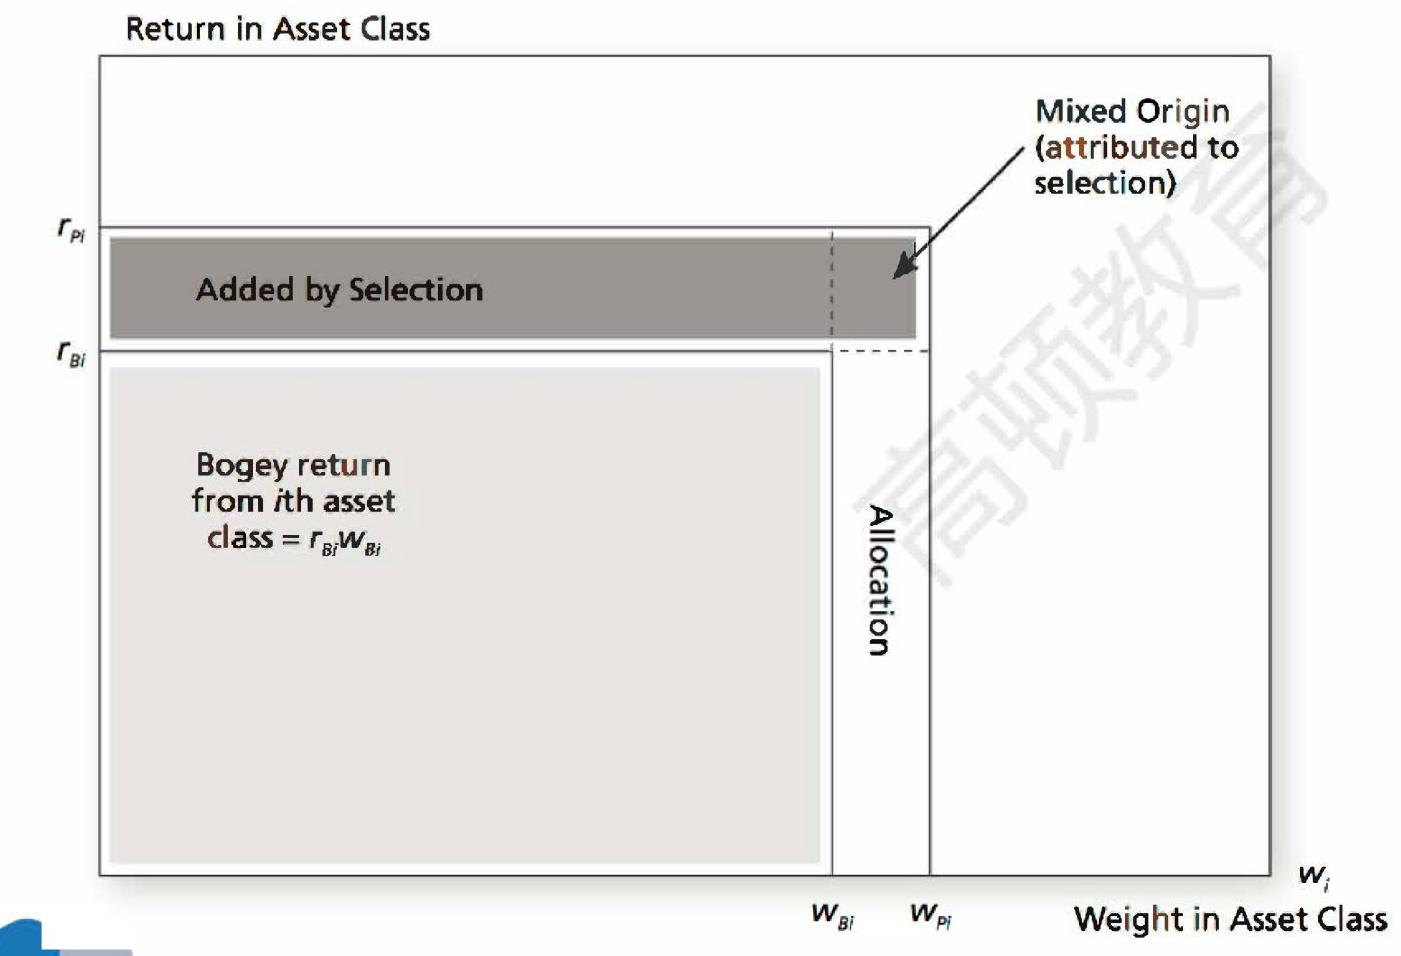
\includegraphics[width=0.4\textwidth]{images/Return in Asset Class.jpg}
    \end{center}    
    
    \begin{table}[H]
    \centering
    \caption{Portfolio Performance Analysis}
    \begin{tabular}{@{}l*{6}{p{2.5cm}@{}}} % 后面6列设置列宽为1.5cm
         & Actual weight & Bench mark weight & Active weight & Portfolio performance(\%) & Return of index(\%) & Excess performance(\%) \\
        \midrule
        Equity & 70\% & 60\% & 10\% & 7.28 & 5.81 & 1.47 \\
        Bonds & 7\% & 30\% & -23\% & 1.89 & 1.45 & 0.44 \\
        Cash & 23\% & 10\% & 13\% & 0.48 & 0.48 & 0 \\
        \bottomrule
    \end{tabular}
    \end{table}
Asset allocation= 0.1·5.81\% + (-0.23)·1.45\% + 0.13·0.48\% =0.003099

Security selection= 0.7·1.47\% + 0.07·0.44\% = 0.0106

\item Example (cont.): sector selection

\begin{table}[h]
    \centering
    \caption{Sector - level Portfolio Performance Analysis}
    \begin{tabular}{@{}l*{5}{p{3cm}@{}}} % 后面5列设置列宽为1.5cm

        \toprule
        \multirow{2}{*}{Sector} & \multicolumn{2}{c}{(1) \newline Beginning of Month Weights (\%)} & (3) & (4) & (5) = (3) × (4) \\
        \cmidrule(lr){2 - 3}
        & Portfolio & S\&P 500 & Active Weights (\%) & Sector Return (\%) & Sector Allocation Contribution \\
        \midrule
        Basic materials & 1.96 & 8.3 & -6.34 & 6.9 & -0.4375 \\
        Business services & 7.84 & 4.1 & 3.74 & 7.0 & 0.2618 \\
        Capital goods & 1.87 & 7.8 & -5.93 & 4.1 & -0.2431 \\
        Consumer cyclical & 8.47 & 12.5 & -4.03 & 8.8 & 0.3546 \\
        Consumer noncyclical & 40.37 & 20.4 & 19.97 & 10.0 & 1.9970 \\
        Credit sensitive & 24.01 & 21.8 & 2.21 & 5.0 & 0.1105 \\
        Energy & 13.53 & 14.2 & -0.67 & 2.6 & -0.0174 \\
        Technology & 1.95 & 10.9 & -8.95 & 0.3 & -0.0269 \\
        \midrule
        TOTAL &  &  &  &  & \underline{1.2898} \\
        \bottomrule
    \end{tabular}
\end{table}

\begin{table}[h]
    \centering
    \caption{Portfolio Performance Decomposition}
    \begin{tabular}{@{}l*{6}{p{2.5cm}@{}}} % 后面6列设置列宽为1.5cm
        \toprule
         & (1) & (2) & (3) & (4) & (5) & (6) \\
         & Actual weight & Benchmark weight & Active weight (1)-(2) & Portfolio performance & Return of index & Excess performance (4)-(5) \\
        \midrule
        Equity & 0.7 & 0.6 & 0.1 & 7.28\% & 5.81\% & 1.47\% \\
        Bonds & 0.07 & 0.3 & -0.23 & 1.89\% & 1.45\% & 0.44\% \\
        Cash & 0.23 & 0.1 & 0.13 & 0.48\% & 0.48\% & 0\% \\
        \midrule

        \multicolumn{3}{c}{} & \multicolumn{3}{c}{} \\
        Asset allocation & \multicolumn{3}{c}{} & \multicolumn{2}{c}{$\sum$(3)$\times$(5)} &  0.3099\% \\
        Selection & \multicolumn{3}{c}{} & \multicolumn{2}{c}{$\sum$(1)$\times$(6)} &  1.060\% \\
        \midrule
        Equity & \multicolumn{2}{c}{} &  1.47\% &  1.47\%*0.7 &  1.0290\% &  \\
        & \multicolumn{2}{c}{-Sector} &  1.29\% & \multicolumn{3}{c}{} \\
        & \multicolumn{2}{c}{-Security} &  0.18\% & \multicolumn{3}{c}{} \\
        Bond & \multicolumn{2}{c}{} &  0.44\% &  0.44\%*0.07 &  0.0308\% &  \\
        \midrule
        \multicolumn{6}{c}{Total alpha} &  1.37\% \\
        \bottomrule
    \end{tabular}
\end{table}

\end{itemize}



